% Chapter 1

\chapter{Introduction} % Main chapter title

\label{Chapter1} % For referencing the chapter elsewhere, use \ref{Chapter1} 

\lhead{Chapter 1. \emph{Introduction}} % This is for the header on each page - perhaps a shortened title

%----------------------------------------------------------------------------------------
% Why are we doing these measurements?
The Internet supports many applications like IoT devices, live video streaming, and online stock trading, with different requirements. The infrastructure and the technologies supporting the internet have advanced, bringing link speeds to hundreds of gigabits per second and packet processing delays to the order of nanoseconds on the latest switching hardware. The evolving landscape has seen increased video traffic~\cite{gipr-sandvine22} and other low-latency-requiring applications. New technologies have been developed and deployed on the internet to cater to the new needs. Google has developed BBR~\cite{bbrgoogle-acmqueue16}, a new CCA to perform better in lossy networks and provide low latencies. Similarly, QUIC~\cite{quic-sigcomm17} is a new user-space transport stack that gives users more flexibility to deploy new CCAs. Recent developments have led to a rapidly evolving congestion control landscape and a need to monitor these new algorithms at the edge to study their impact on the network.

Designing new algorithms for the network for tasks like congestion control and active queue management requires us to be aware of many network hyper-parameters like flow size, flow duration, number of concurrent flows and RTT distribution amongst others. Our best estimates of these metrics are quite outdated~\cite{tcprtt-imc03,revisittcp-imc21,2004-shakkottai-t20}, and their measurements must be replenished in correspondence to the changing Internet landscape. The campus of NUS serves as a unique vantage point in the measurement of these key metrics. Since in most cases, the bottleneck lies near the client (edge of the network), these measurements will be helpful in the development of future congestion control algorithms.
The measurements will also help diagnose potential network issues like microbursts/heavy hitters, buffer overflows, and increases in latencies. It aids in facilitating the network operator to have fine-grained network metrics to resolve various other problems associated with the campus network. 

% What are we doing?
In this thesis, we describe the design and implementation of a testbed that will allow us to measure several important parameters of flows that are part of the traffic going through the campus' gateway router. We use these measurement to detect congestion events by measuring link utilization, packet losses and the RTT values of the flows part of the congested links.

% How are we doing?
\section{Experimental Setup}

We deploy our passive measurement testbed to study and monitor live internet traffic at the edge of our campus network. The vantage point that meets this criterion and offers maximum insight into the network would be the links connecting the gateway router of the campus network.

\begin{figure}[t]
    \centering
        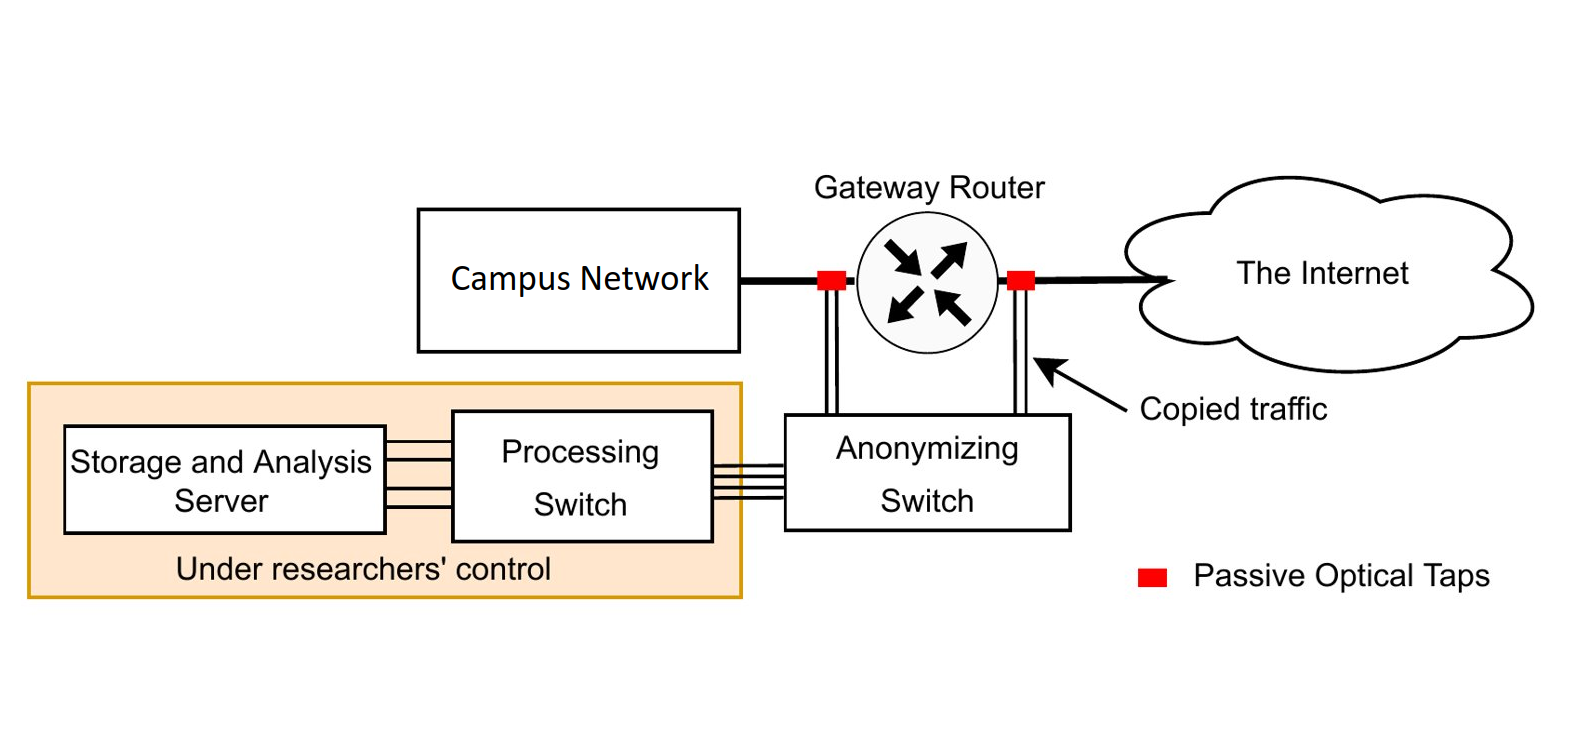
\includegraphics[width=\textwidth]{Figures/setup.png}
    \caption[Experimental Setup]{Experimental Setup}
    \label{fig:setup}
    \bigskip
\end{figure}

Figure \ref{fig:setup} shows how we tap live traffic from the network links connecting our campus to the internet. The gateway router is connected to the campus network using 10G optical links. We tap the links using a passive optical tap to obtain a copy of the traffic at the line rate. The device splits the optical signal into two identical copies without affecting the rate of the traffic. The mirrored traffic is passed across to the anonymizing switch. The anonymizing switch has been used to ensure the privacy of the users and is under the control of the network operators. The anonymizing switch anonymizes the packet by encrypting the source and destination IP addresses and TCP ports by a custom anonymization mechanism. It also truncates the TCP/UDP payload. After doing this, it adds a custom header in between the Ethernet and IP headers of the packet to preserve some telemetry information of the packet such as packet length, packet timestamp, and header length. It then forwards the anonymized packets to the processing switch. The processing switch then passes the uplink and downlink traffic to different ports on the storage analysis server to do different computations on the traffic.

\section{Packet Structure}

\begin{figure}[t]
    \centering
        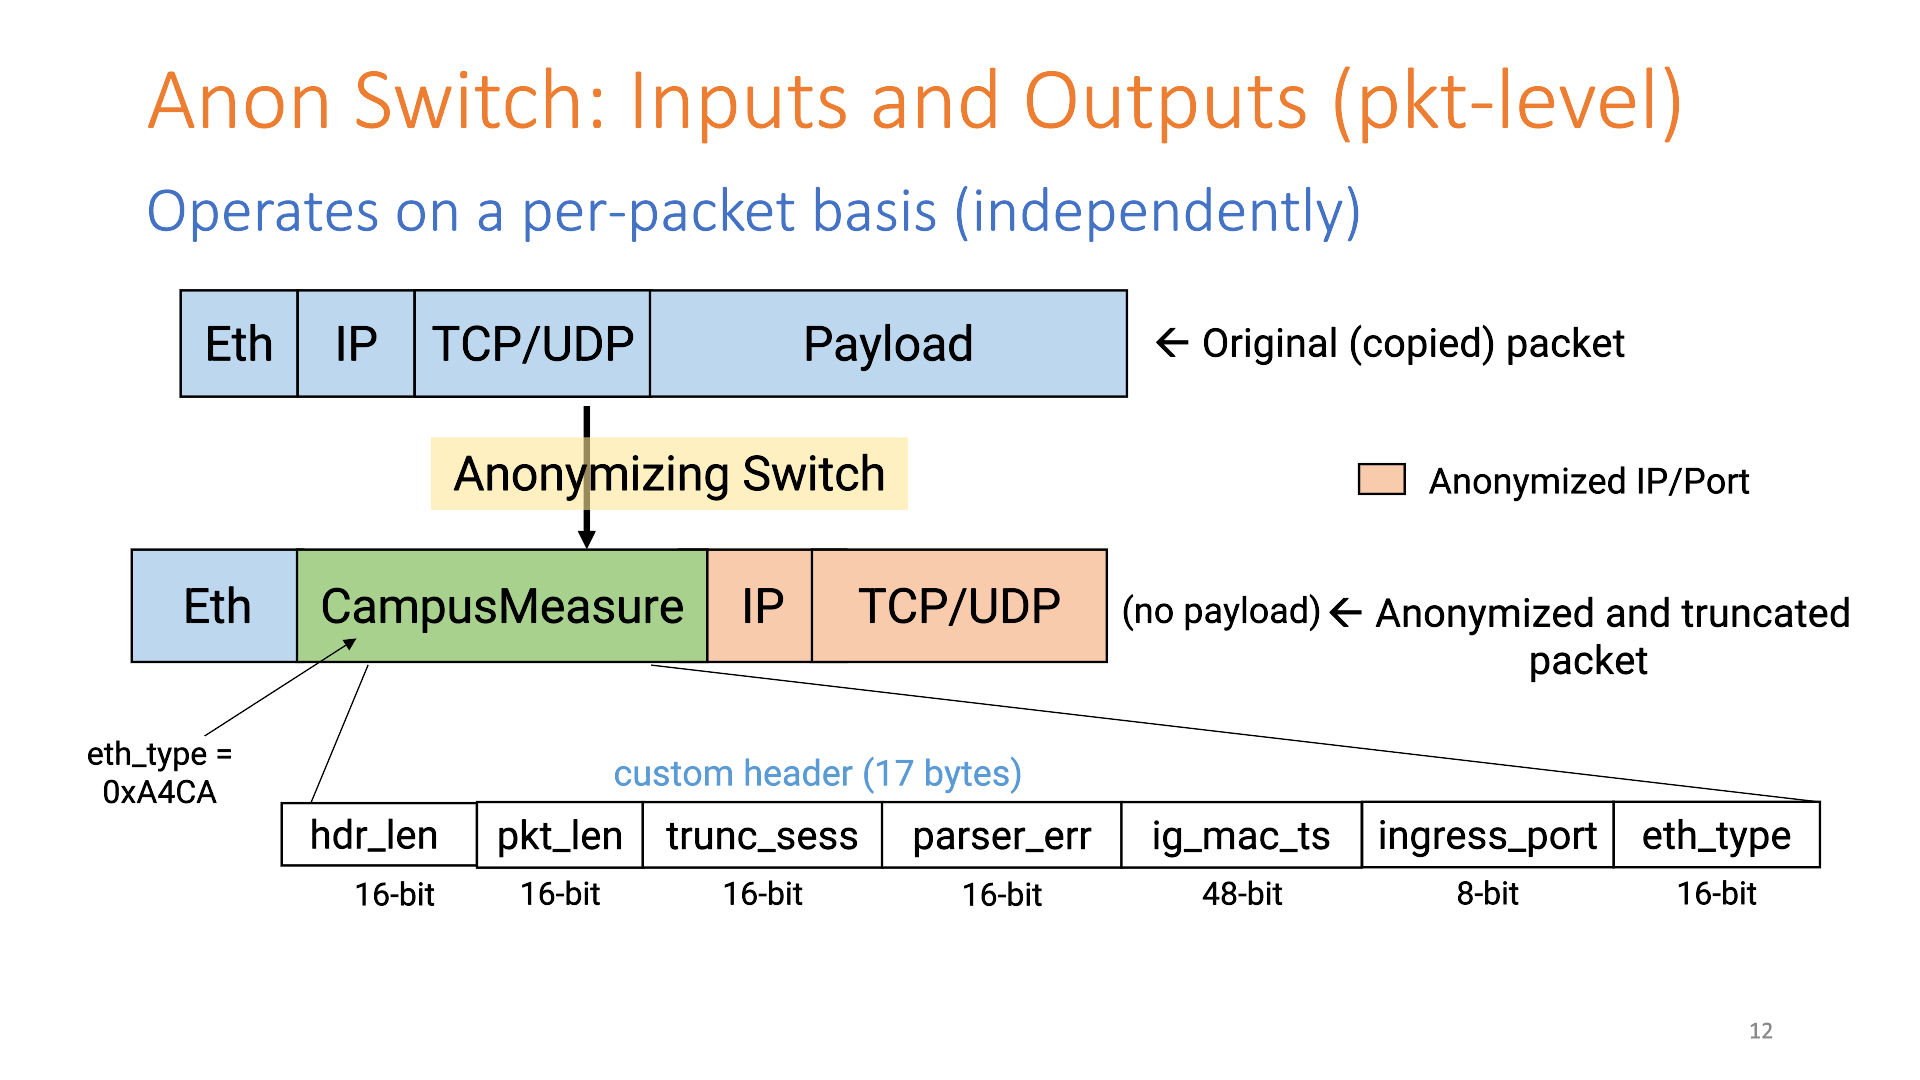
\includegraphics[width=\textwidth]{Figures/pkt-struct.png}
    \caption[Packet structure]{Packet structure}
    \label{fig:struct}
    \bigskip
\end{figure}

Figure \ref{fig:struct} shows the structure of the packet after anonymization by the switch. It inserts a new header field of 17 bytes called the CampusMeasure Header in between the Ethernet and the IP fields.
The most important fields in this new header are the $hdr\_len,pkt\_len$ and $ig\_mac\_ts$ fields. The ingress mac time-stamp is recorded as the packet is received at the ingress port of the switch. The packet length is the total length of the packet before the truncation. These two fields are used to do most of our computations in the later sections such as calculating the link utilization, flow duration etc.

\section{Packet capture at the server}

Traditional packet capture tools such as tcpdump~\cite{tcpdump} operate in the kernel space of the operating system. The functioning of these tools involve context switching between the user and kernel space which adds additional overhead. This overhead causes latency and can lead to packet drops in an environment involving high packet rates. These tools also generally use inefficient memory management techniques compromising system performance.

\begin{figure}[t]
    \centering
        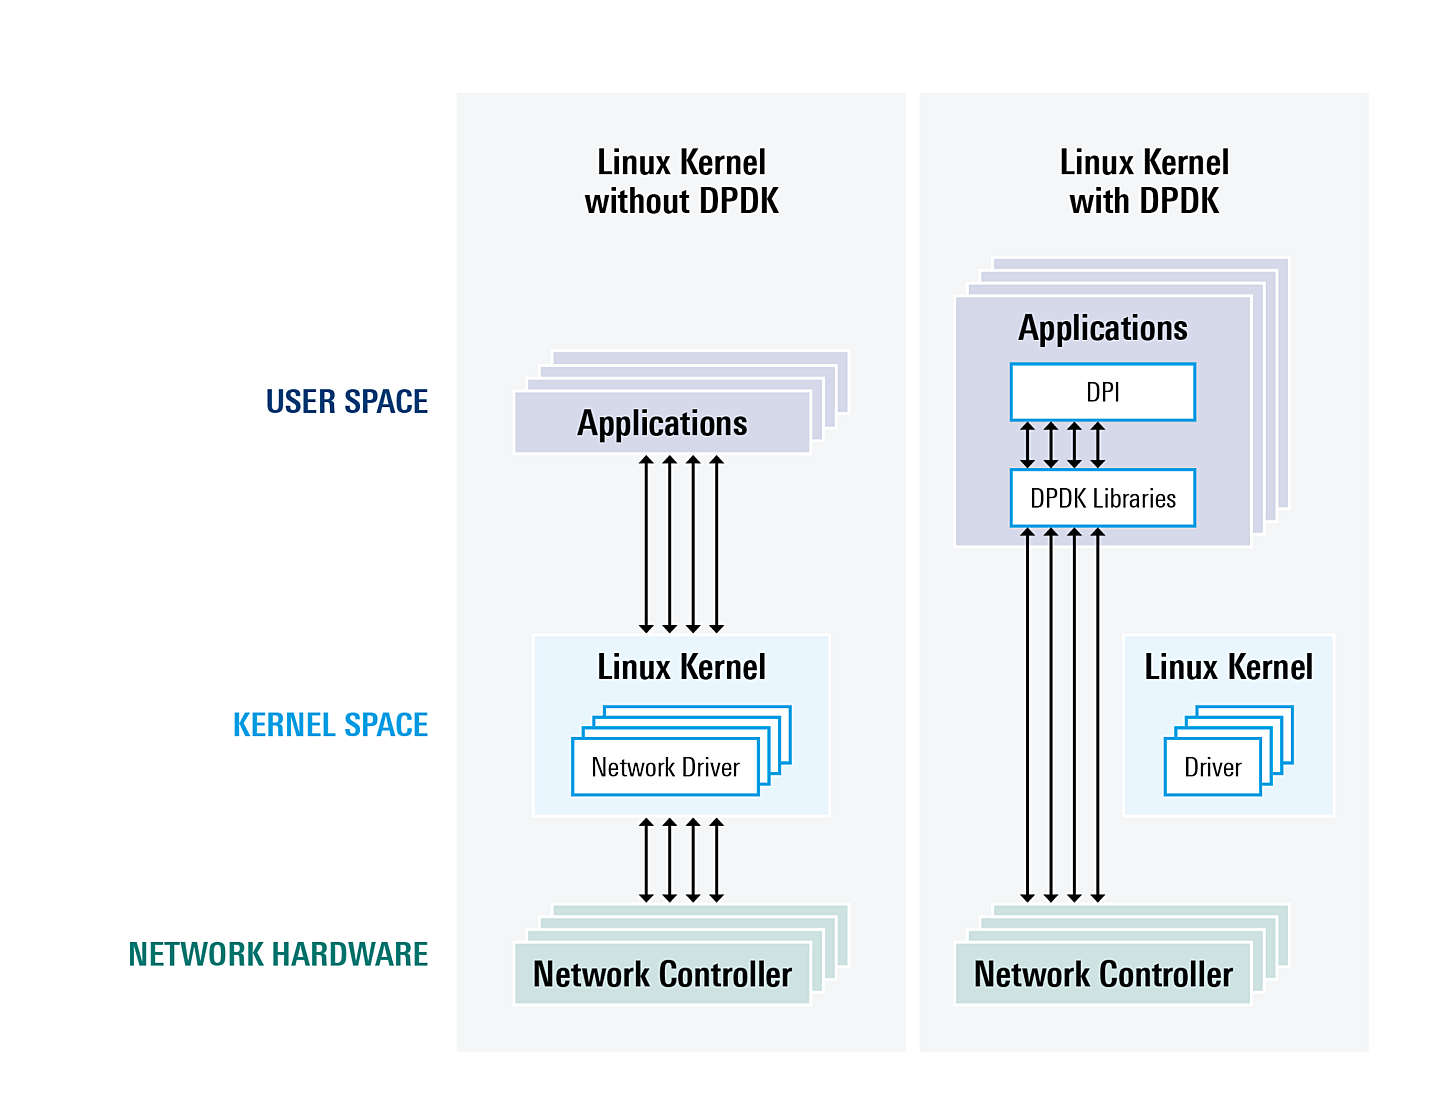
\includegraphics[width=\textwidth]{Figures/dpdk.png}
    \caption[DPDK Approach]{DPDK Approach ~\cite{dpdk2023}}
    \label{fig:dpdk}
    \bigskip
\end{figure}

Instead of these traditional tools, we use DPDK~\cite{dpdk} to capture packets at high rates efficiently. As shown in Figure \ref{fig:dpdk}, DPDK bypasses the operating system kernel and directly accesses network hardware. As a result of bypassing the kernel space, and handling packet processing in the user space itself, DPDK achieves lower latency and can capture packets without any drops even at rates such as 10 Gbps. We write a packet capture program in C using DPDK libraries to capture traffic from the two ports of the server simultaneously using two worker threads and write the captured packets to two separate pcap files.

We then modify the tool to customize packet captures. We can input the duration of packet capture, the frequency after which to start the next capture, and the start and end times of the packet capture, and the packet capture would run to create separate pcap files(uplink and downlink) for each capture.
%----------------------------------------------------------------------------------------